%% OJEPN article template for LaTeX
%% Licence: Creative Commons Attribution Share-Alike 4.0
%% Author:  Andy J. Wills
%% Adapted from a Creative Commons template by Jonathan Baron

\documentclass[twocolumn]{article}
\usepackage[utf8]{inputenc}
\usepackage[T1]{fontenc}
\usepackage[english]{babel}
\usepackage{ifpdf,amsmath,amsthm,amssymb,amsfonts,newtxtext,newtxmath} 
\usepackage{array,graphicx,dcolumn,multirow,hevea,abstract,hanging}
\usepackage[labelfont=sc,textfont=sf]{caption}
\usepackage[colorlinks=true,linkcolor=black,anchorcolor=black,citecolor=black,filecolor=black,menucolor=black,runcolor=black,urlcolor=black,hyperfootnotes=false,breaklinks=true]{hyperref}
\urlstyle{rm}
\usepackage[hyphenbreaks]{breakurl}
%\usepackage{natbib} % must come afer hyperfootnotes
%\setlength{\bibsep}{0pt}
\usepackage{booktabs} % \toprule \midrule \bottomrule \cmidrule(lr){a-b}
% define centered and ragged columns:
\newcolumntype{L}[1]{>{\raggedright\arraybackslash }p{#1}} % can use m{}
\newcolumntype{C}[1]{>{\centering\arraybackslash }p{#1}}
\newcolumntype{R}[1]{>{\raggedleft\arraybackslash }p{#1}}
\newcolumntype{d}[1]{D{.}{.}{#1}} % d{3.2} for 3 places on l, 2 on r
\newcommand{\mc}{\multicolumn}
\topmargin=-.3in \oddsidemargin=-.1in \evensidemargin=-.1in \textheight=9in \textwidth=6.8in
\setlength\tabcolsep{1mm}
\setlength\columnsep{5mm}
\setlength\abovecaptionskip{1ex}
\setlength\belowcaptionskip{.5ex}
\setlength\belowbottomsep{.3ex}
\setlength\lightrulewidth{.04em}
\renewcommand\arraystretch{1.2}
\renewcommand{\topfraction}{1}
\renewcommand{\textfraction}{0}
\renewcommand{\floatpagefraction}{.9}
% \renewcommand{\baselinestretch}{1.00} \large\normalsize % for fixing spaces
\widowpenalty=1000
\clubpenalty=1000
\setlength{\parskip}{0ex}
\let\tempone\itemize
\let\temptwo\enditemize
\let\tempthree\enumerate
\let\tempfour\endenumerate
\renewenvironment{itemize}{\tempone\setlength{\itemsep}{0pt}}{\temptwo}
\renewenvironment{enumerate}{\tempthree\setlength{\itemsep}{0pt}}{\tempfour}

%%%%%%%%%%%%%%%%%%%%%%%%%%%%%%%%%%%%%%%%%%%%%%%%%%%%%%%%%%%%%%%%%%%%%
\setcounter{page}{1} % start with first page

\title{Example title}

\author{
Stuart G. Smith\thanks{School of Psychology, University of Plymouth, U.K. Email: stuart.smith@ply.ac.uk}
\and 
  Andy J. Jones\footnotemark[1] % indicates same as 1st thanks
}

\date{} % leave empty
\begin{document} % goes here

% fill in short title
\newcommand{\jhead}{Submitted to OJEPN, 20XX}
\newcommand{\jdate}{Vol.~X}
\pagestyle{myheadings} \markright{\protect\small \jhead, \jdate \hfill SHORT TITLE \qquad}
\begin{htmlonly}
\end{htmlonly}
%\begin{latexonly}
\twocolumn[
\vspace{-.3in}
{\small \jhead, \jdate, pp.\ XX--XX \hfill \url{https://doi.org/10.46221/ojepn.xxxx.xxxx}}
%\end{latexonly}

\maketitle

%\begin{latexonly}
\vspace{-3mm}
\begin{onecolabstract}
%\end{latexonly}
  Place abstract here.
  
\smallskip
\noindent
Keywords: INSERT KEYWORDS

%\begin{latexonly}
\end{onecolabstract}\bigskip
]
%\end{latexonly}

{\renewcommand{\thefootnote}{}
\footnotetext{ % note blank lines above and below acknowledgment
Copyright: \copyright\ 2021.
The authors license this article under the terms of the
\href{http://creativecommons.org/licenses/by/3.0/}{Creative Commons
  Attribution Share-Alike 4.0 License.}
}}

\saythanks

\setlength{\baselineskip}{12pt plus.2pt}

\section{Example section heading}


\begin{equation}
  \Delta V_{x} = \alpha_{x}L(\lambda-V_{x})
\end{equation}

\begin{figure}[t!]
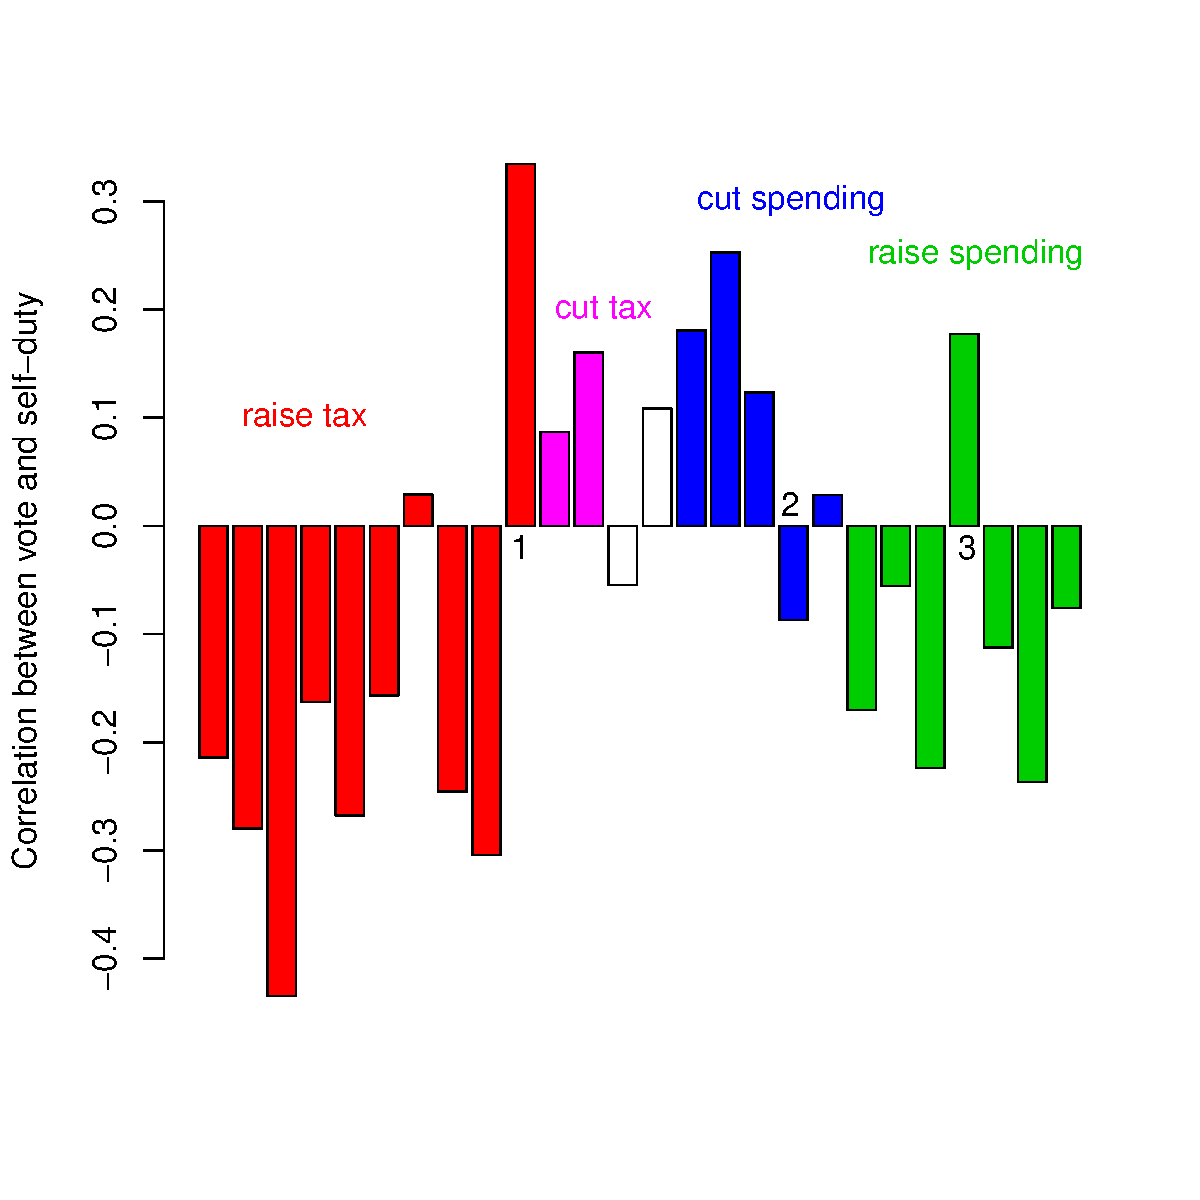
\includegraphics[width=\columnwidth]{dut11.pdf}
\caption{Example figure}
\end{figure}

\subsection{Example sub-heading}

\begin{table}[b!]
	\begin{center}
	\caption{Example table}
	\label{table:ply043CategoryParameters}
		\begin{tabular}[b]{c c c c c c}
			\hline\noalign{\smallskip}
			& \multicolumn{2}{c}{Height} & \multicolumn{2}{c}{Length} &\\
			& $\mu$ & $\sigma$ & $\mu$ & $\sigma$ & $cov_{xy}$ \\
			\noalign{\smallskip}\hline\noalign{\smallskip}
						\multicolumn{5}{l}{Conjunction} \\
			\noalign{\smallskip}
			A & 0.3 & 0.12 & 0.8 & 0.12 \\
			B & 0.3 & 0.12 & 0.4 & 0.12 \\ 
			B & 0.7 & 0.12 & 0.4 & 0.12 \\
			B & 0.7 & 0.12 & 0.8 & 0.12 \\
			\multicolumn{5}{l}{Information-integration} \\
			A & 3.1562 & 0.667 & 66.5 & 12.247 & 5\\
			B & 4.7546 & 0.667 & 37 & 12.247 & 5\\
			\noalign{\smallskip}\hline
		\end{tabular}
	\end{center}
\end{table}

\section*{References}

\begin{hangparas}{1em}{1}

Ashby, F. G., Alfonso-Reese, L. A., \& Waldron, E. M. (1918). Example reference.
\emph{Psychological Preview, 105}(3), 442-481.
\url{https://doi.org/10.1037/0034-295x.105.3.244}

\end{hangparas}

\end{document}

%%% Local Variables:
%%% mode: latex
%%% TeX-master: t
%%% End:

